\chapter{The Single Skill That Built His \$100M Year Business}

This chapter reads the interview as a practical model of wealth creation rather than as a transcript of slogans. Johnny Anton is presented by School of Hard Knocks as a salesman and entrepreneur whose path runs from hardship to high-revenue businesses; the claims below remain tied to that interview testimony. There are no validated mathematical screenshots for this lecture, so the diagrams and formulas are cautious reconstructions of the mechanisms Johnny describes: failure, feedback, pattern recognition, ownership risk, talent, and sales psychology.

\section{The Portable Skill}

The opening establishes Johnny Anton as a witness. He is introduced as the child of Iraqi immigrants, raised in a poor part of Detroit, homeless for two years, and later involved in scaling multiple businesses past nine figures in revenue. The point of the opening is not only biographical. It sets up a claim about portability.

A market can crash. Crypto can fall. Fraud can appear. But the interview frames sales as a skill that can be carried into any business with sufficient demand. In that sense, sales is not treated merely as persuasion. It is treated as a revenue-producing operator: a repeatable way of turning demand, attention, product, and human certainty into cash flow.

A compact way to record the claim is

\begin{equation}
\text{portable wealth skill}
\quad \approx \quad
\text{ability to create revenue under changing conditions}.
\end{equation}

This is not an equation written on a board. It is a faithful abstraction of the opening claim. The interview begins with this because the rest of the conversation asks what sort of person, practice, and business system can make such a skill durable.

\section{Failure Without Significance}

The first question is about advice to a younger self. Johnny's answer is direct: fail faster, and do not make failure mean something final about the self. The rhythm matters. He does not start with tactics. He starts with the emotional interpretation of a bad result.

We can model the basic learning loop as

\begin{equation}
A_t \longrightarrow R_t \longrightarrow L_t \longrightarrow A_{t+1},
\end{equation}

where \(A_t\) is the action at time \(t\), \(R_t\) is the result, and \(L_t\) is the lesson extracted from that result. The dangerous extra term is not the failure itself. It is the identity-level significance placed on the failure.

Let \(S_t\) denote the significance load attached to a result. Then the practical claim is not that failure disappears, but that learning accelerates when \(S_t\) is reduced:

\begin{equation}
S_t \downarrow
\quad \Longrightarrow \quad
\text{faster extraction of } L_t
\quad \Longrightarrow \quad
\text{faster next action } A_{t+1}.
\end{equation}

Johnny connects this to a claim about startup culture: failing forward intelligently, learning from mistakes, compounding time, and removing the significance of everything. Whether the country-level comparison is externally verified is not the point for the chapter. The transcript uses it as a motivation for a local rule: a result should become information before it becomes identity.

\subsection{Question \& Answer}

\paragraph{Question.}
Why does failing faster matter if failure still costs time, money, or reputation?

\paragraph{Answer.}
Because the cost of failure is not only the external loss. It is also the delay created when a person turns a result into a verdict about the self. In the interview's operating logic, the loop should be

\begin{equation}
\text{attempt}
\rightarrow
\text{result}
\rightarrow
\text{lesson}
\rightarrow
\text{next attempt},
\end{equation}

not

\begin{equation}
\text{attempt}
\rightarrow
\text{result}
\rightarrow
\text{identity collapse}
\rightarrow
\text{delay}.
\end{equation}

The first loop compounds. The second loop stalls.

\section{The Three Habits}

After the advice about failure, the interviewer asks for the habits that led to becoming a millionaire. Johnny gives three, and their order is important.

First, he names meditation and describes it as reconditioning the mind. He says he had been meditating consistently for over six years and traces an early exposure to wrestling camp, where meditation was tied to winning a state championship. He then broadens the claim: every idea starts in imagination. His example is Walt Disney imagining Disney World before it existed materially, facing banker refusals, and pursuing a project he describes as requiring a \( \$5 \) million loan and later costing \( \$15 \) million.

This should be written as an interview claim, not as a scientific theorem about the subconscious. Its role in the lecture is to introduce the idea that action depends on what a person can first permit as possible.

Second, Johnny moves to consistent action and documentation. This is the most operational habit. He says his sales team uses an end-of-day report: who they talked to, what happened, what worked, what did not work, and who they were being behind what they said.

Third, he says to cut checks quickly and pay people who already have the desired results. The mechanism is pattern recognition: do not reinvent the wheel; learn the patterns of people who have already produced the outcome.

We can summarize the three-part structure as

\begin{align}
\text{Habit 1} &: \text{recondition identity and possibility},\\
\text{Habit 2} &: \text{act, measure, and revise},\\
\text{Habit 3} &: \text{buy proximity to proven patterns}.
\end{align}

The second and third habits are where the chapter's mathematical structure is strongest. They turn self-improvement into iteration and pattern recognition.

\section{Feedback Loops Beat Scripts}

Johnny's most precise operating mechanism is the end-of-day report. A salesperson makes calls. The result is observed. The result is written down. The next behavior is adjusted. Then the loop repeats.

\begin{equation}
\text{Calls}_t
\longrightarrow
\text{Report}_t
\longrightarrow
\text{Adjustment}_t
\longrightarrow
\text{Calls}_{t+1}.
\end{equation}

The report itself has fields:

\begin{equation}
\text{Report}_t =
\{
\text{contacts},
\text{result},
\text{worked},
\text{did not work},
\text{state/context}
\}.
\end{equation}

The last field is crucial. Johnny does not only ask what words were said. He asks who the salesperson was being behind the words. That is his way of distinguishing content from context.

\subsection{Question \& Answer}

\paragraph{Question.}
If two salespeople use the same script, why does one outperform the other?

\paragraph{Answer.}
The transcript's answer is that content is not the whole system. The same words can be delivered from different states, different levels of certainty, different listening quality, and different interpretations of the buyer. A cautious model is

\begin{equation}
O =
f(
\text{offer},
\text{prospect},
\text{script},
\text{context},
\text{salesperson state}
),
\end{equation}

where \(O\) is the sales outcome. The script is only one input. Johnny's point is that the hidden inputs often dominate the visible words.

\subsection{A Worked Update Rule}

Let \(c_t\) be the number of meaningful sales conversations in a day, \(w_t\) the set of observed behaviors that worked, \(n_t\) the set that did not work, and \(q_t\) a qualitative description of the salesperson's state. The report can be treated as

\begin{equation}
\text{Report}_t = (c_t,w_t,n_t,q_t).
\end{equation}

The next day's action plan is not guessed from motivation alone. It is updated from the report:

\begin{equation}
A_{t+1}
=
U(A_t,\text{Report}_t),
\end{equation}

where \(U\) is the practical update rule: keep what worked, remove or test what did not, and adjust the state behind the action.

In a simple example, suppose a salesperson makes \(c_t=20\) calls. The report says that direct price talk caused resistance, while asking about the prospect's current constraint opened the conversation. Then the next action plan is

\begin{align}
A_t &: \text{lead with price and offer},\\
\text{Report}_t &: \text{resistance high; diagnosis questions worked},\\
A_{t+1} &: \text{lead with current problem, then bridge to offer}.
\end{align}

This is the lecture's practical mathematics: not a numerical formula, but an explicit learning rule.

\begin{figure}
\centering
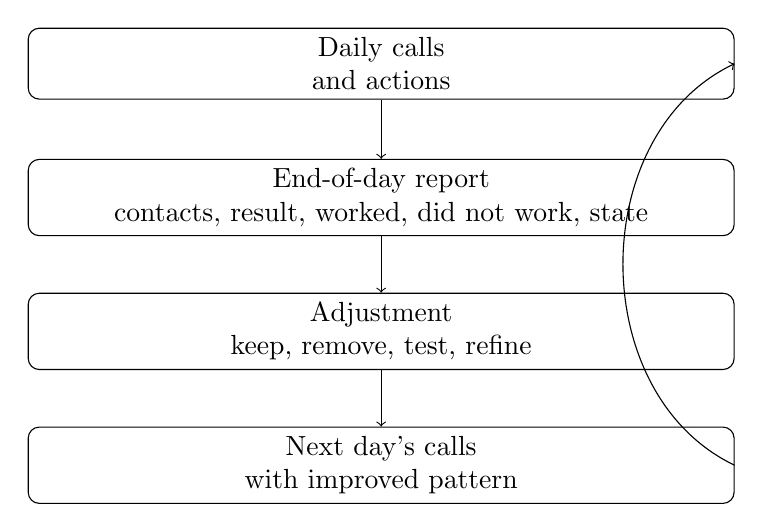
\begin{tikzpicture}
\node[draw, rounded corners, text width=0.72\linewidth, align=center] (calls) at (0,0) {Daily calls\\and actions};
\node[draw, rounded corners, text width=0.72\linewidth, align=center] (report) at (0,-1.7) {End-of-day report\\contacts, result, worked, did not work, state};
\node[draw, rounded corners, text width=0.72\linewidth, align=center] (adjust) at (0,-3.4) {Adjustment\\keep, remove, test, refine};
\node[draw, rounded corners, text width=0.72\linewidth, align=center] (next) at (0,-5.1) {Next day's calls\\with improved pattern};

\draw[->] (calls) -- (report);
\draw[->] (report) -- (adjust);
\draw[->] (adjust) -- (next);
\draw[->] (next.east) .. controls (2.6,-4.2) and (2.6,-0.9) .. (calls.east);
\end{tikzpicture}
\caption{The interview's implied sales feedback loop. The diagram is reconstructed from the transcript; no validated board diagram was available.}
\end{figure}

\section{Pattern Recognition And Paid Proximity}

The third habit is to pay people who already have the results one wants. Johnny says to cut checks faster and bigger, not as consumption, but as access to pattern recognition. The phrase ``success leaves clues'' becomes a practical rule: if a person has already solved a problem, do not treat ignorance as originality.

The local model is stimulus and response:

\begin{equation}
S \longrightarrow R.
\end{equation}

In sales, \(S\) may be something said by the salesperson, an offer made, a question asked, or a frame introduced. \(R\) is the prospect's response. Pattern recognition is the skill of seeing which stimuli repeatedly produce which responses, in which contexts.

\begin{definition}
In these notes, pattern recognition means the ability to observe repeated stimulus-response structures in business situations and to model the actions of people who already produce the desired result.
\end{definition}

The transcript uses wrestling, school, and sales as examples of the same method. Johnny says he reached a state championship after only two years of wrestling and performed well in school by studying what had to be done in the moment-to-moment phenomenon. The broad claim is that business action has patterns, and those patterns can be observed, purchased, modeled, and practiced.

This section also explains why meditation returns later in the discussion. Johnny claims that if a person remains trapped in an old identity, information from books and podcasts does not convert into action. Again, the chapter should treat that as Johnny's claim, not as established psychology. But structurally it matters: identity determines whether the pattern is adopted or sabotaged.

\section{Ego, Risk, And The Missing Business Functions}

The interview then pivots from habit to ego. Johnny gives a reversal: because he helped a company move from high eight figures toward multiple nine figures, he thought starting his own business would be easy. His boss Paul challenged that assumption. A half-million dollars in \(100\%\) commission sales income did not require Johnny to carry every business function.

The warning can be decomposed as

\begin{equation}
\text{Business ownership}
=
\text{sales}
+
\text{marketing}
+
\text{delivery}
+
\text{hiring}
+
\text{operations}
+
\text{finance}
+
\text{risk}.
\end{equation}

A top closer may master one term in this sum and still underestimate the whole expression. This is the section's central distinction.

\begin{remark}
The transcript's anecdote should not be reduced to humility as a mood. Its commercial mechanism is sharper: commission sales can hide the full system of business risk. Ownership exposes the missing terms.
\end{remark}

Johnny attributes part of his early arrogance to wanting to prove his father wrong and to not giving up an old identity. The chapter should preserve this as an anecdote about motive, but the practical rule is simpler: pay someone who has the result, give up the need to figure everything out alone, and learn where the blind spots are.

\section{Scaling Beyond Sales}

The next question asks what takes a business from seven to eight figures and from eight to nine. Johnny cites Ryan Breslow as a model and says the answer comes down to fundraising and recruiting. He then broadens the point: scaling requires cash, hiring, leadership, vision, compensation, talent, and a strong product.

A narrow chain captures the claim:

\begin{equation}
\text{Product}
\longrightarrow
\text{Vision and leadership}
\longrightarrow
\text{Fundraising and recruiting}
\longrightarrow
\text{Talent}
\longrightarrow
\text{Scale}.
\end{equation}

The order is important. In Johnny's account, one cannot attract good leaders without a good product. One cannot attract talent without compensation packages. One cannot sustain compensation without a product that sells. The enterprise is not a single lever; it is a coupled system.

\begin{figure}
\centering
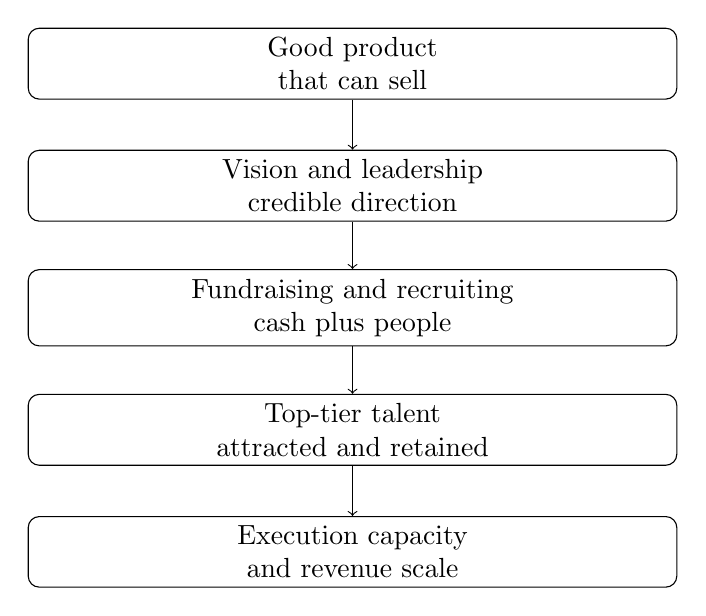
\begin{tikzpicture}
\node[draw, rounded corners, text width=0.66\linewidth, align=center] (product) at (0,0) {Good product\\that can sell};
\node[draw, rounded corners, text width=0.66\linewidth, align=center] (vision) at (0,-1.55) {Vision and leadership\\credible direction};
\node[draw, rounded corners, text width=0.66\linewidth, align=center] (fund) at (0,-3.1) {Fundraising and recruiting\\cash plus people};
\node[draw, rounded corners, text width=0.66\linewidth, align=center] (talent) at (0,-4.65) {Top-tier talent\\attracted and retained};
\node[draw, rounded corners, text width=0.66\linewidth, align=center] (scale) at (0,-6.2) {Execution capacity\\and revenue scale};

\draw[->] (product) -- (vision);
\draw[->] (vision) -- (fund);
\draw[->] (fund) -- (talent);
\draw[->] (talent) -- (scale);
\end{tikzpicture}
\caption{A transcript-grounded reconstruction of Johnny's scale chain.}
\end{figure}

This is the point where the interview shifts from the individual closer to the business builder. Sales still matters, but it is no longer sufficient by itself.

\section{Starting From Zero}

The interviewer then asks what Johnny would do if his bank account went to zero. The answer begins with survival: sell the most expensive thing available until rent, food, and shelter are covered. Johnny explicitly connects this to basic needs. Once survival is stabilized, the next move is not luxury. It is value creation.

The rebuild sequence is

\begin{equation}
\begin{aligned}
&\text{sell expensive offer}
\rightarrow
\text{food and shelter}
\rightarrow
\text{free value}
\rightarrow
\text{testimonials and case studies}\\
&\rightarrow
\text{anchor client}
\rightarrow
\text{adjacent prospects}
\rightarrow
\text{high-value low-risk package}
\rightarrow
\text{sales team and lead sources}.
\end{aligned}
\end{equation}

This sequence belongs in the dynamic book's chapters on first money-making mechanisms, customer problem, distribution, risk, and scale. It is one of the clearest operational passages in the interview.

\begin{enumerate}
\item First, find a high-ticket offer and sell it to restore cash.
\item Then use skills and connections to add value for free.
\item Convert free value into testimonials, case studies, and an anchor client.
\item Use that proof to sell adjacent customers in the same niche or nearby markets.
\item Package the offer with high value and low perceived risk for the client.
\item Build a sales team and increase lead sources.
\end{enumerate}

The mechanism is proof before scale. The anchor client creates a local witness, and that witness makes the next sale easier.

\section{Sales As Transfer Of Certainty}

The final sales question asks how to turn a no into a yes. Johnny reframes the premise. The better question is not how to overcome objections after they appear, but how to understand the buyer well enough that many objections are prevented in the presentation itself.

He divides buyer understanding into demographics and psychographics. Demographics describe who the prospect is: age, background, origin, family situation, and similar facts. Psychographics describe how the prospect thinks, behaves, desires, fears, and decides.

\begin{table}
\centering
\begin{tabular}{|p{0.42\linewidth}|p{0.42\linewidth}|}
\hline
\textbf{Demographics} & \textbf{Psychographics} \\
\hline
Age, background, origin, family context, life situation & Interests, desires, behavior, fears, psychology, decision pattern \\
\hline
Who the person is in observable terms & How the person interprets problems and makes choices \\
\hline
\end{tabular}
\caption{A compact reconstruction of Johnny's distinction between demographic and psychographic understanding.}
\end{table}

His definition of sales can be written as a bridge:

\begin{equation}
\text{current situation}
\xrightarrow{\text{product/service plus certainty}}
\text{desired situation}.
\end{equation}

\subsection{Question \& Answer}

\paragraph{Question.}
How do we turn a no into a yes?

\paragraph{Answer.}
In Johnny's framing, we should not begin with the objection. We begin with the person. We understand where the buyer is, where the buyer wants to go, and what the buyer cares about. Then the offer is not pushed as our agenda; it is presented as the bridge from current state to desired state.

That gives the final model:

\begin{equation}
\text{Sales}
=
\text{diagnosis}
+
\text{certainty}
+
\text{credible bridge}.
\end{equation}

The diagnosis comes from listening. The certainty comes from the salesperson's own psychology and understanding of the offer. The credible bridge is the product or service positioned against the buyer's stated problem.

\section{Summary}

This interview is not a mathematics lecture in the usual sense, and there are no validated board equations or diagrams. Its structure is nevertheless highly procedural. Johnny begins with sales as a portable skill, then moves through failure, identity, feedback loops, pattern recognition, ego, enterprise risk, talent, starting from zero, and sales psychology.

The central operating rule is iteration with reduced emotional drag:

\begin{equation}
A_t \rightarrow R_t \rightarrow L_t \rightarrow A_{t+1}.
\end{equation}

The strongest business mechanism is the feedback loop:

\begin{equation}
\text{action}
\rightarrow
\text{measurement}
\rightarrow
\text{adjustment}
\rightarrow
\text{improved action}.
\end{equation}

And the final sales mechanism is the bridge from a customer's current situation to a desired one. The chapter should preserve the interview's source-conscious quality: Johnny's anecdotes remain anecdotes, his claims remain attributed claims, and the mechanisms are extracted carefully from the order in which he gives them.